\chapter{Occupation Resolved Conductance in the Mixed-Valence Regime}\label{cha:mixed_valence_conductance}


\begin{figure}[ht]
  \begin{center}
%% includegraphics: comment the following if not using the graphicx package
    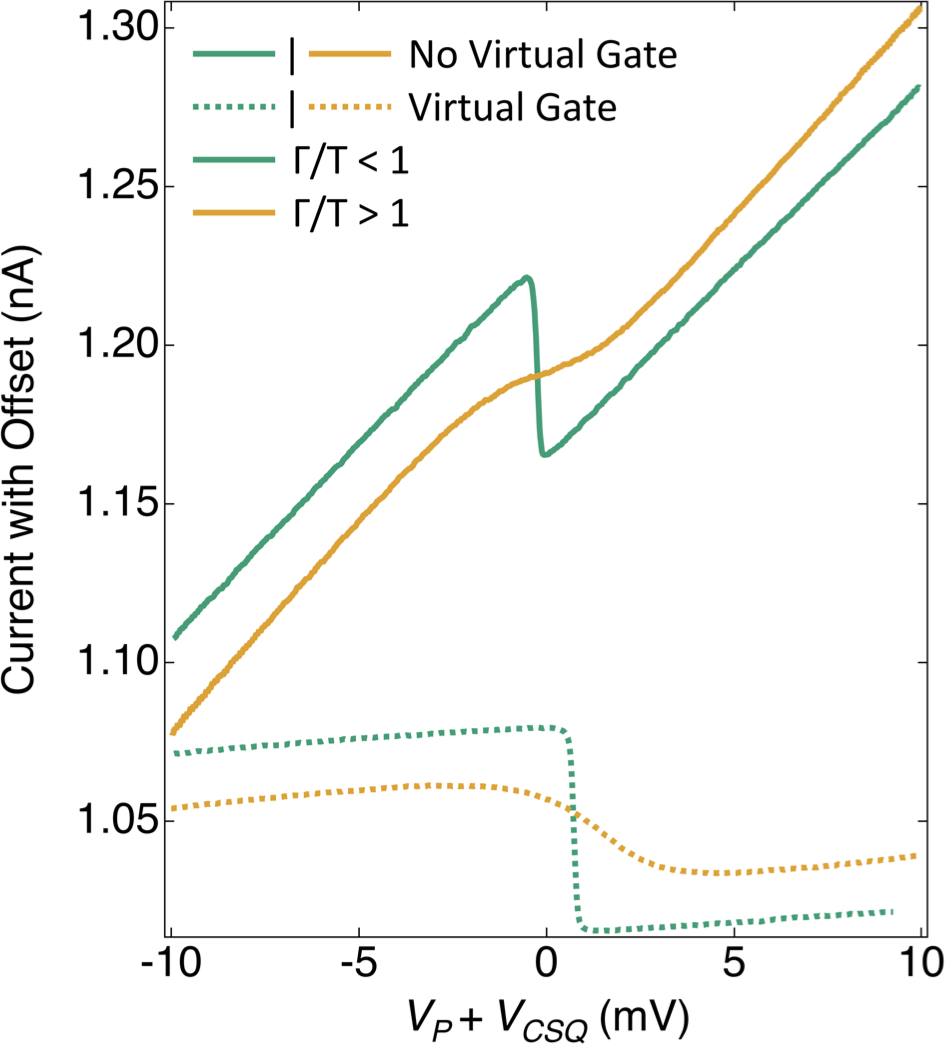
\includegraphics[width=0.8\textwidth]{figures/ch3/crop_PosterFiguresMaster.009.png}
    \caption[Measuring charge transitions with and without a virtual gate]{\label{fig:ch3/virtual_gate_example} 
    % For some options that work with pdf\LaTeX, please see this discussion:
    %   \url{http://tex.stackexchange.com/questions/11839}.  
    Data of a weakly (green) and strongly (yellow) coupled charge transition scanned with a single gate V\textsubscript{P} (solid line) and a virtual gate  V\textsubscript{P}~+~V\textsubscript{CSQ} (dashed line). The traces have been offset in current for ease of comparison. V\textsubscript{P} has a large effect on the dot energy, however, it also changes other parameters due to capacitive coupling. Here, a virtual gate is used to change the dot energy whilst keeping the current through the charge sensor constant. This helps with visually identifying strongly coupled charge transitions which become very broadened. More importantly, the charge sensor stays in the linear regime where changes in the potential are linearly proportional to changes in the current. Note the x-axis is only showing the value of V\textsubscript{P}. As V\textsubscript{P} is swept negative to positive, V\textsubscript{CSQ} is swept positive to negative.}
  \end{center}
\end{figure}


\begin{figure}[ht]
  \begin{center}
%% includegraphics: comment the following if not using the graphicx package
    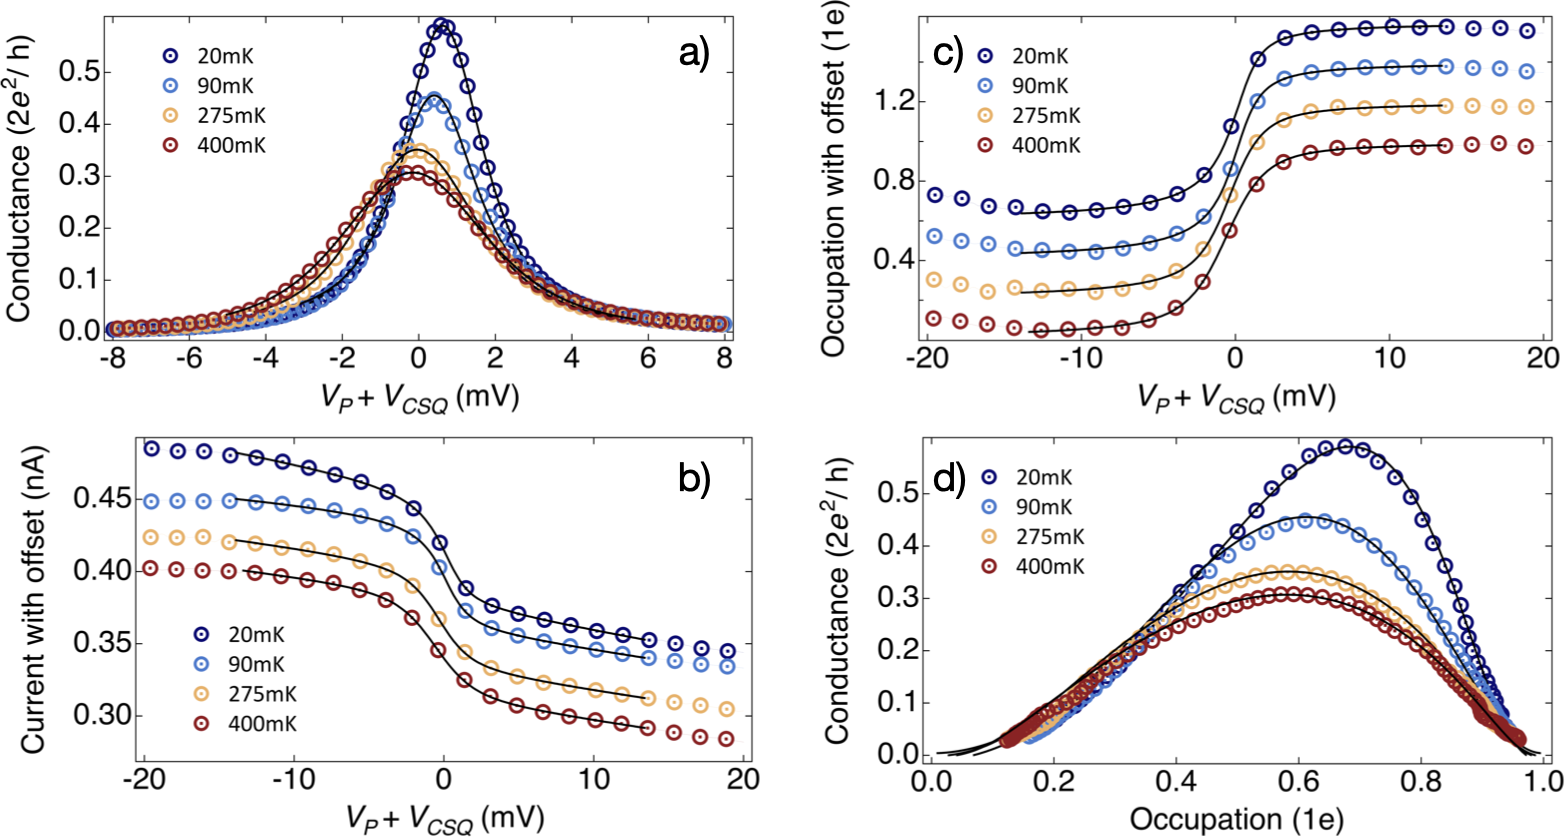
\includegraphics[width=1\textwidth]{figures/ch3/crop_PosterFiguresMaster.010.png}
    \caption[Method to determine gamma and leverarm and show Kondo enhancement of conductance in the mixed-valence regime]{\label{fig:ch3/cond_occ_gf} 
    % For some options that work with pdf\LaTeX, please see this discussion:
    %   \url{http://tex.stackexchange.com/questions/11839}.  
    (\textbf{a}) Conductance data as a single electron enters a strongly coupled ($\mathrm{\Gamma/T > 1}$) quantum dot at four different temperatures. The x location of the conductance maxima has not been shifted, it is the original x location of the acquired data. The fits (in grey) are from a global fit to NRG, where the gamma and leverarm parameters are held fixed across all four temperatures. (\textbf{b}) Charge transitions are measured simultaneously with the conductance. The charge transitions are fit to NRG where the gamma and leverarm parameters are held fixed to the values determined from the global fit to conductance. (\textbf{c}) Charge transitions are converted to occupation by removing the relevant fit parameters. These are amplitude, current offset, cross capacitance of virtual gate and occupation dependant cross capacitance. (\textbf{d}) A plot of conductance vs. occupation helps show the enhanced conductance due to Kondo.}
  \end{center}
\end{figure}



\begin{figure}[ht]
  \begin{center}
%% includegraphics: comment the following if not using the graphicx package
    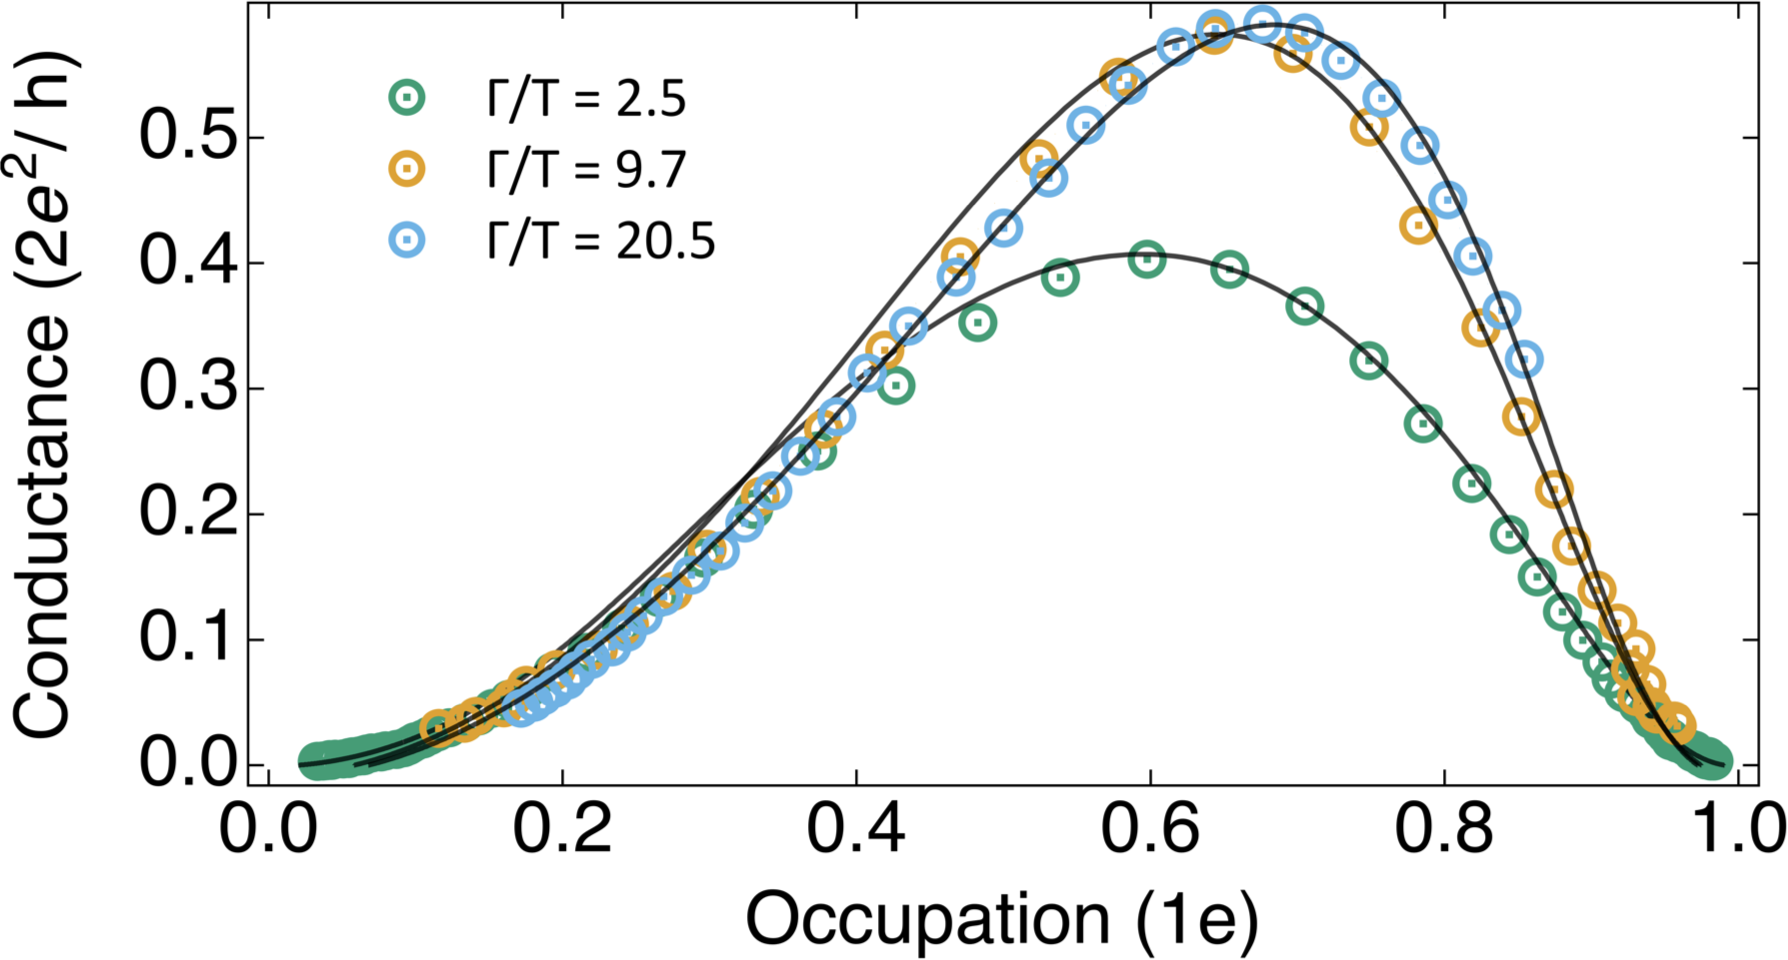
\includegraphics[width=1\textwidth]{figures/ch3/crop_PosterFiguresMaster.011.png}
    \caption[Conductance vs. Occupation : Varying the coupling strength between the quantum dot and leads]{\label{fig:ch3/cond_occ_couplingstrength} 
    % For some options that work with pdf\LaTeX, please see this discussion:
    %   \url{http://tex.stackexchange.com/questions/11839}.  
    Conductance vs. occupation in a weak (green) and strong (blue) coupling regime. Each trace is taken at \qty{20}{mK}. The coupling strength $\mathrm{\Gamma/T}$ was determined from a global fit to multiple temperatures. The NRG (grey) conductance vs. occupation corresponding to the determined $\mathrm{\Gamma/T}$ is plotted ontop of the data where good agreement is found at each coupling strength.}
  \end{center}
\end{figure}


\begin{figure}[ht]
  \begin{center}
%% includegraphics: comment the following if not using the graphicx package
    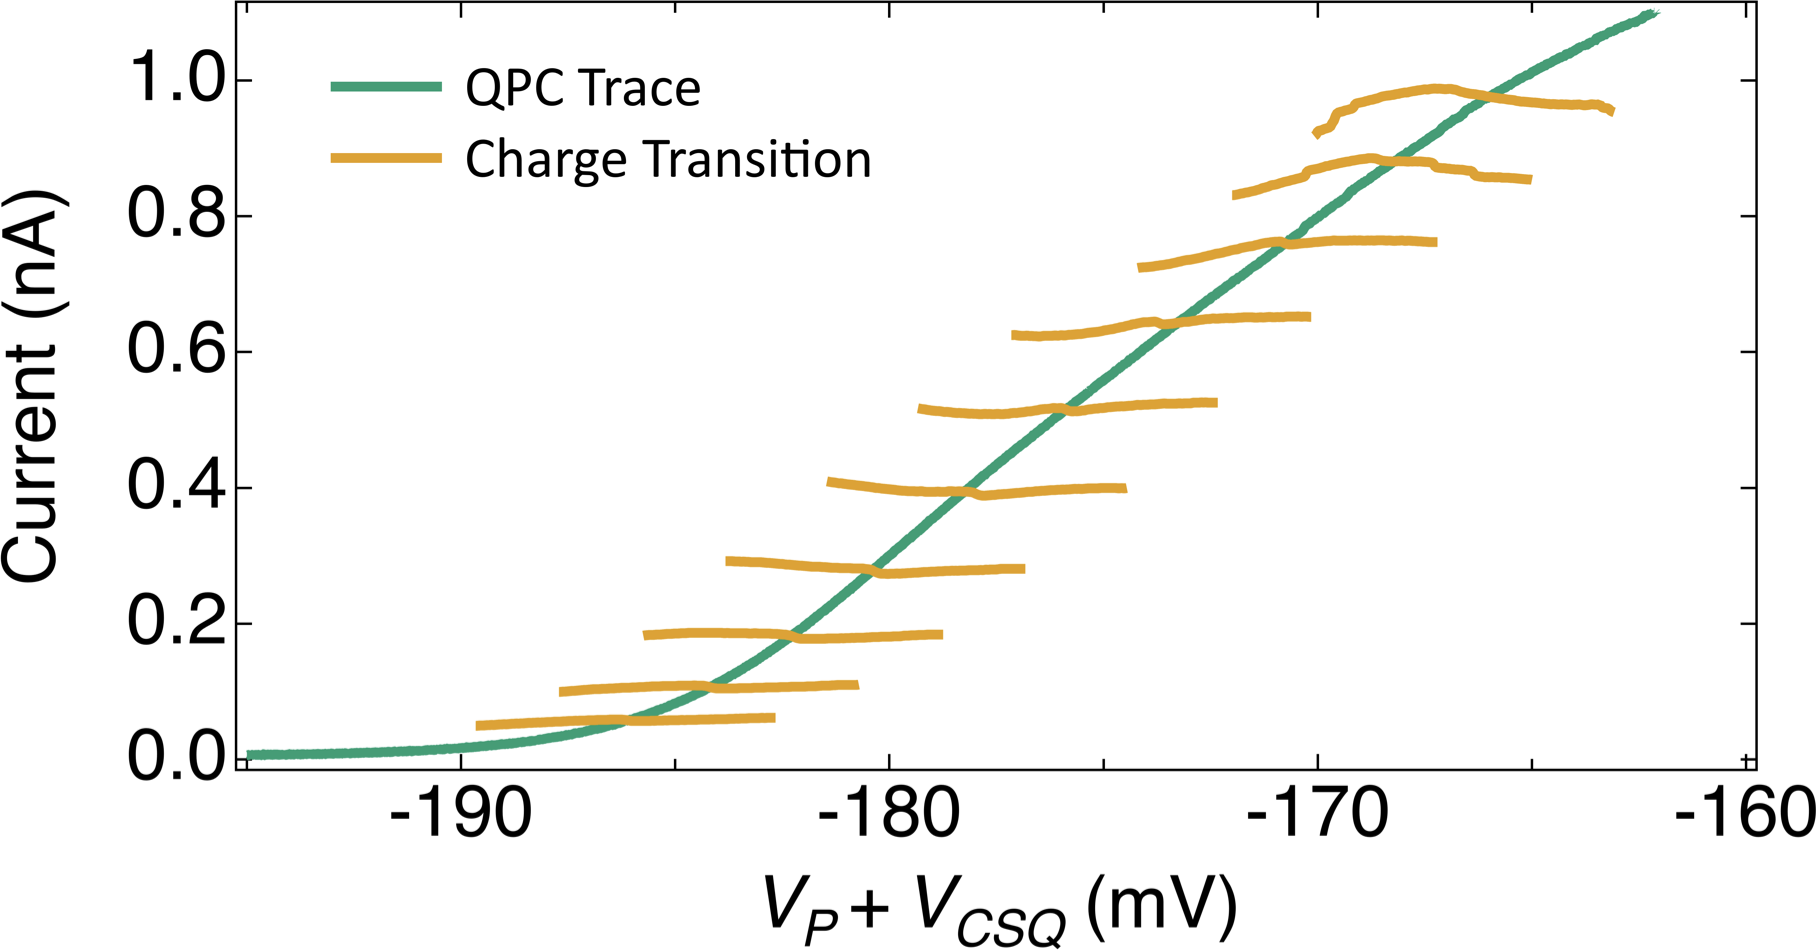
\includegraphics[width=1\textwidth]{figures/ch3/crop_PosterFiguresMaster.012.png}
    \caption[Charge transitions measured at various current set points through the charge sensor]{\label{fig:ch3/cond_occ_ct_setpoints} 
    % For some options that work with pdf\LaTeX, please see this discussion:
    %   \url{http://tex.stackexchange.com/questions/11839}.  
    Current through the charge sensor (green) from pinch off to the start of the first conductance plateau. Corresponding charge transition (yellow) at each of the current set-points through the charge sensor. Note the x-axis is not the same between the underlying QPC trace and charge transitions. The charge transitions have been scaled the same amount x-axis for visual purposes. As the current through the charge sensor is changed the charge transition vary dramatically, with the left and right slopes curving upwards, downwards, in the same direction or opposite to each other.}
  \end{center}
\end{figure}


\begin{figure}[ht]
  \begin{center}
%% includegraphics: comment the following if not using the graphicx package
    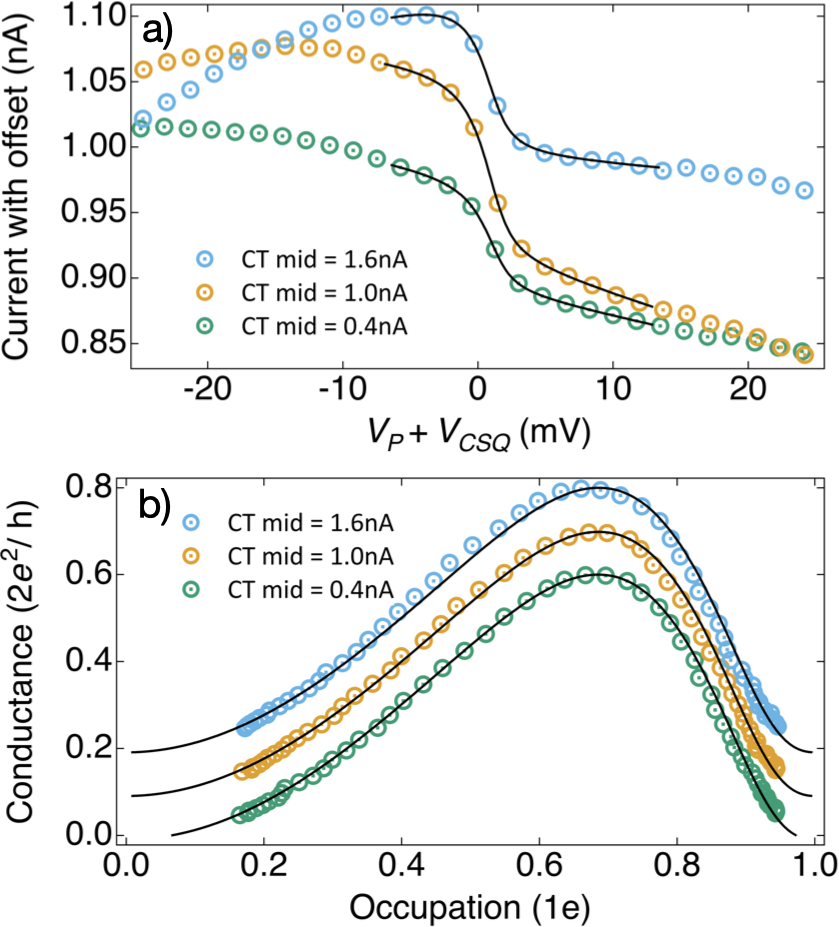
\includegraphics[width=0.8\textwidth]{figures/ch3/crop_PosterFiguresMaster.013.png}
    \caption[Conductance vs. Occupation : Varying the current through the charge sensor]{\label{fig:ch3/cond_occ_QPC_vs_ct} 
    % For some options that work with pdf\LaTeX, please see this discussion:
    %   \url{http://tex.stackexchange.com/questions/11839}.  
    (\textbf{a}) Charge transitions measured with high (blue) and low (green) current through the charge sensor. The transition are offset in current for ease of comparison. The x-axis uses the same virtual gate for each charge transition. The slopes on either side of the charge transitions vary with current through the charge sensor indicating the optimal virtual gate also changes. (\textbf{b}) Conductance vs. occupation ($\mathrm{\Gamma/T=21}$) at different currents through the charge sensor. The traces are offset for clarity. Each trace is taken at \qty{20}{mK}. The coupling strength $\mathrm{\Gamma/T}$ was determined from a global fit to multiple temperatures. The NRG (grey) conductance vs. occupation corresponding to the determined $\mathrm{\Gamma/T}$ is plotted on-top of the data where good agreement is found for each current set-point.}
  \end{center}
\end{figure}



\begin{figure}[ht]
  \begin{center}
%% includegraphics: comment the following if not using the graphicx package
    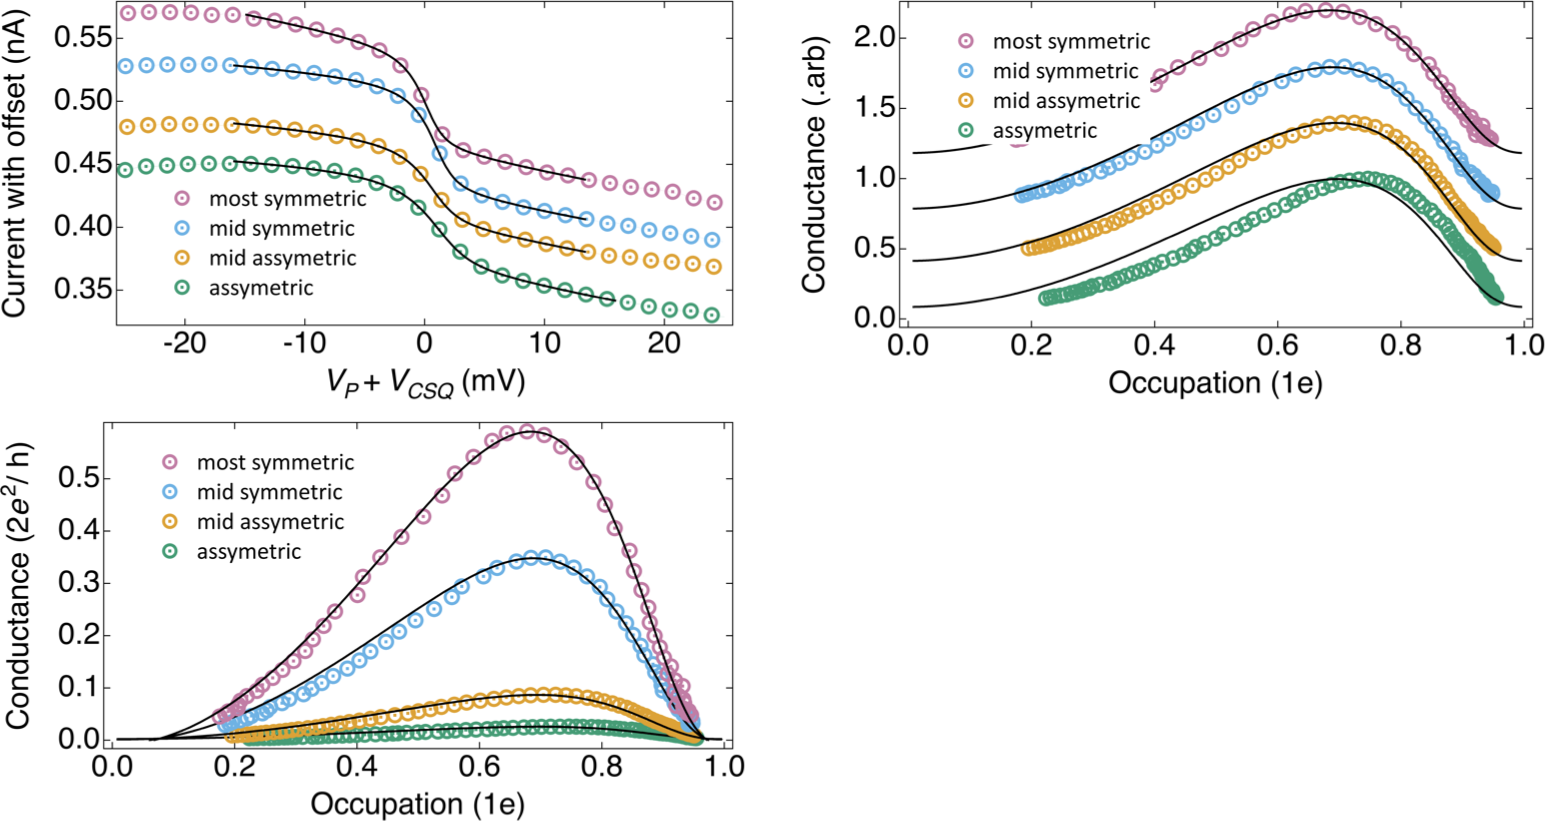
\includegraphics[width=1\textwidth]{figures/ch3/crop_PosterFiguresMaster.014.png}
    \caption[Conductance vs. Occupation : Varying the coupling symmetry between quantum dot and leads]{\label{fig:ch3/cond_occ_assymetry} 
    % For some options that work with pdf\LaTeX, please see this discussion:
    %   \url{http://tex.stackexchange.com/questions/11839}.  
    (\textbf{a}) Charge transitions measured with high (blue) and low (green) current through the charge sensor. The transition are offset in current for ease of comparison. The x-axis uses the same virtual gate for each charge transition. The slopes on either side of the charge transitions vary with current through the charge sensor indicating the optimal virtual gate also changes. (\textbf{b}) Conductance vs. occupation ($\mathrm{\Gamma/T=21}$) at different currents through the charge sensor. The traces are offset for clarity. Each trace is taken at \qty{20}{mK}. The coupling strength $\mathrm{\Gamma/T}$ was determined from a global fit to multiple temperatures. The NRG (grey) conductance vs. occupation corresponding to the determined $\mathrm{\Gamma/T}$ is plotted on-top of the data where good agreement is found for each current set-point.}
  \end{center}
\end{figure}